\documentclass{ctexbeamer}
\usepackage{amsmath,amssymb}
\usepackage{amsthm}
\usepackage{subfig}
\usepackage{graphicx}
\usepackage[defaultmono,scale=0.85]{droidsansmono}
% \usepackage{tikz}
\usepackage{minted}
\usepackage{color}
% \usepackage{mdframed}
% \usepackage[colorlink=true,xetex]{hyperref}

\usetheme{Madrid}
\usefonttheme[onlymath]{serif}
\definecolor{codebg}{rgb}{0.95,0.95,0.95}
\setCJKmonofont{WenQuanYi Micro Hei Mono}
% \surroundwithmdframed{minted}

\setminted{bgcolor=codebg,autogobble,breaklines}
\setmintedinline{bgcolor=codebg}

\newcommand{\theauthor}{Sparky\_14145}
\newcommand{\theinst}{College of Software Engineering}
\newcommand{\theshortinst}{CoSE}

\input{personal_info/info.tex}

\author{\theauthor}
\institute[\theshortinst]{\theinst}
\title{CTF 新挑战}
\subtitle{第五章 Linux 二进制分析}

\begin{document}
    \begin{frame}
        \titlepage
    \end{frame}

    \begin{frame}
        \frametitle{目录}
        \tableofcontents
    \end{frame}

    \section{准备工作}
    \begin{frame}[fragile]
        \frametitle{准备工作}
    
        准备二进制加载器等的过程省略。\pause

        尝试运行 \texttt{oracle} 可执行文件时得到以下错误:

        \begin{minted}{zsh}
            ./oracle: error while loading shared libraries: libcrypto.so.1.0.0: cannot open shared object file: No such file or directory
        \end{minted}
        \pause
        在网上搜索 \texttt{libcrypto.so.1.0.0},发现它是 OpenSSL 的一部分,且版本较低。打开终端,执行:

        \begin{minted}{zsh}
            sudo pacman -S openssl-1.0
        \end{minted}

        问题解决。
    
    \end{frame}

    \section{Level 3}

    \begin{frame}[fragile]
        \frametitle{Level 3}
        \framesubtitle{提示}
    
        \mintinline{zsh}{oracle} 给出的提示是:\pause

        \begin{minted}{text}
            Fix four broken parts
            修复四处错误
        \end{minted}

        \pause
        但是到底要修复哪里的哪四处错误?不知道...
    
    \end{frame}

    \begin{frame}[fragile]
        \frametitle{Level 3}
        \framesubtitle{确认文件类型} 
    
        运行 \mintinline{zsh}{file lvl3},得到如下结果:\pause

        \begin{minted}{text}
            lvl3-origin: ELF 64-bit LSB executable, Motorola Coldfire, version 1 (Novell Modesto), can't read elf program headers at 4022250974, for GNU/Linux 2.6.32, BuildID[sha1]=b6c0e8d914c6433e661b2cac794108671bdcaa06, stripped
        \end{minted}
        \pause

        又是摩托罗拉 ColdFire,又是被收购的 Novell,还有 Modesto,乱七八糟的,肯定是哪里出问题了。
    
    \end{frame}

    \begin{frame}[fragile]
        \frametitle{Level 3}
        \framesubtitle{进一步确认文件信息}
    
        运行 \mintinline{zsh}{readelf -h lvl3},得到以下信息:

        {
            \tiny
            \begin{minted}[highlightlines={6,9,21}]{text}
                ELF 头:
                Magic:  7f 45 4c 46 02 01 01 0b 00 00 00 00 00 00 00 00 
                类别:                              ELF64
                数据:                              2 补码,小端序 (little endian)
                Version:                           1 (current)
                OS/ABI:                            Novell - Modesto
                ABI 版本:                          0
                类型:                              EXEC (可执行文件)
                系统架构:                          Motorola Coldfire
                版本:                              0x1
                入口点地址:                       0x4005d0
                程序头起点:                       4022250974 (bytes into file)
                Start of section headers:          4480 (bytes into file)
                标志:                             0x0
                Size of this header:               64 (bytes)
                Size of program headers:           56 (bytes)
                Number of program headers:         9
                Size of section headers:           64 (bytes)
                Number of section headers:         29
                Section header string table index: 28
                readelf:错误:Reading 504 bytes extends past end of file for 程序头
            \end{minted}
        }
        
        \pause 从输出中我们可以确定三处错误。
    
    \end{frame}

    \begin{frame}[fragile]
        \frametitle{Level 3}
        \framesubtitle{修复已知的三处}
    
        使用 Vim 直接修改二进制文件:\pause

        使用命令 \mintinline{vim}{:%!xxd} 将文件变为 \mintinline{text}{xxd} 输出的结果:

        \begin{center}
            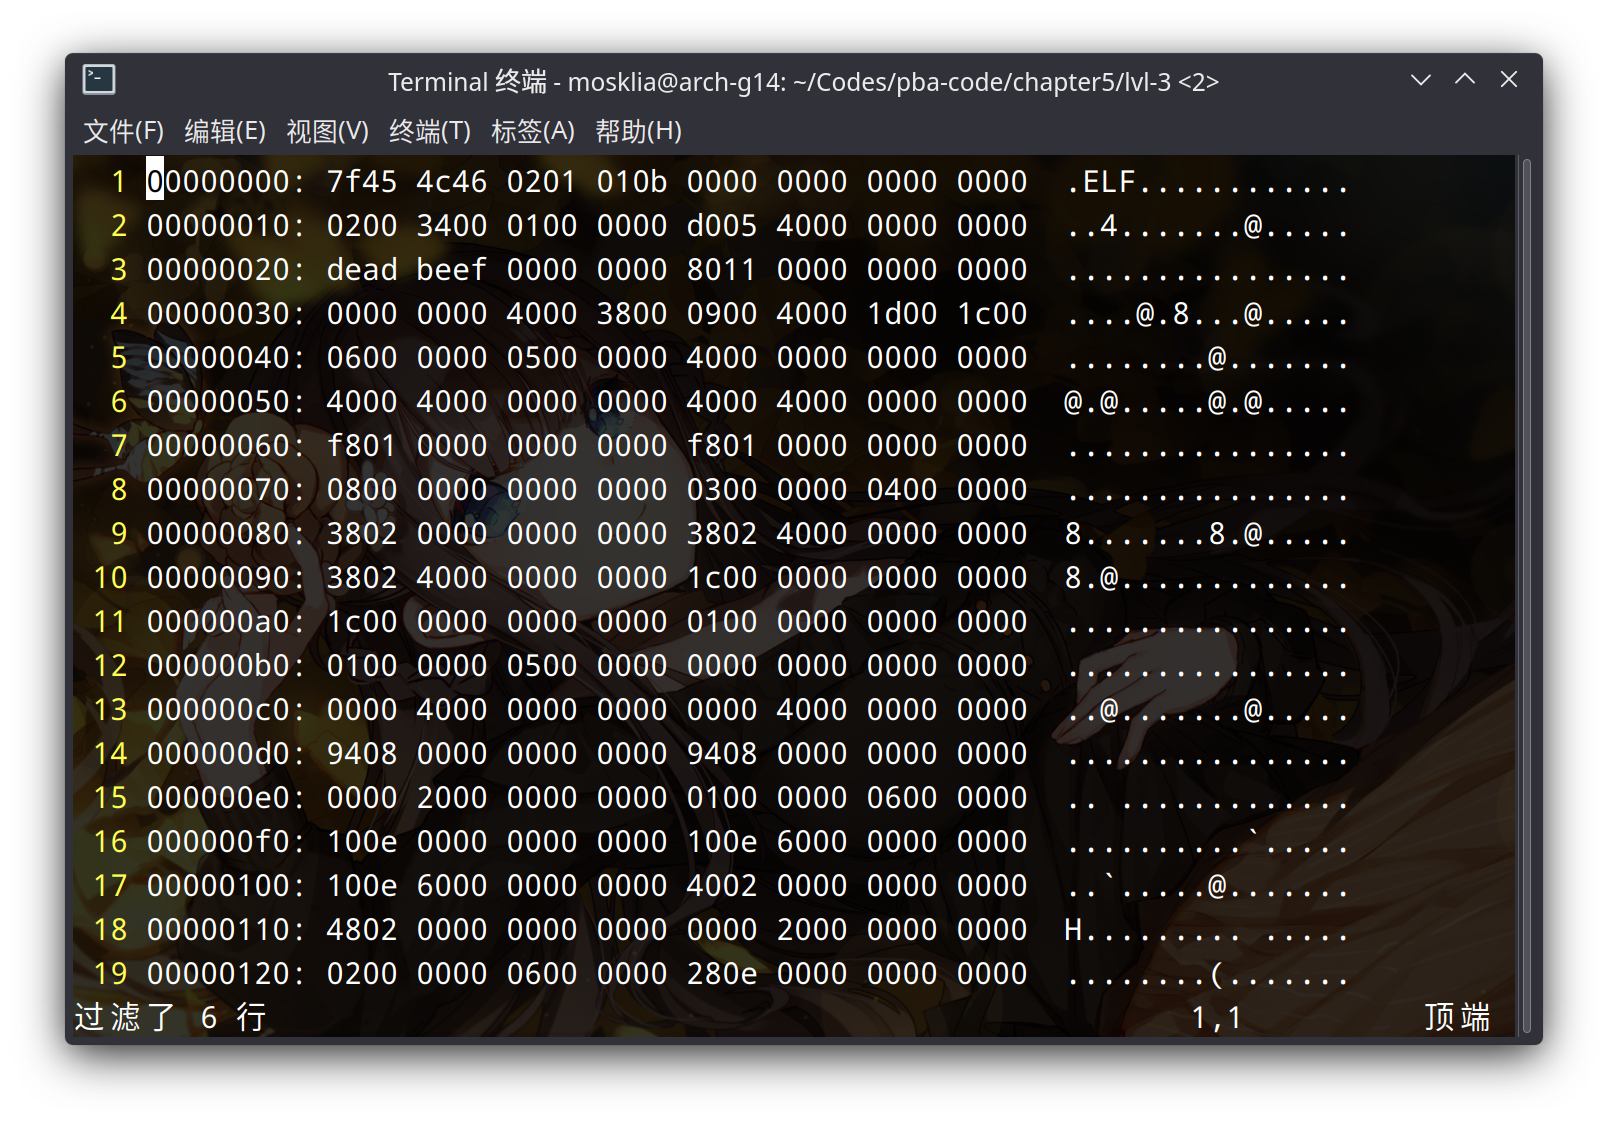
\includegraphics[width=0.45\textwidth]{pics/lvl3-vim-1.png}\;\pause
            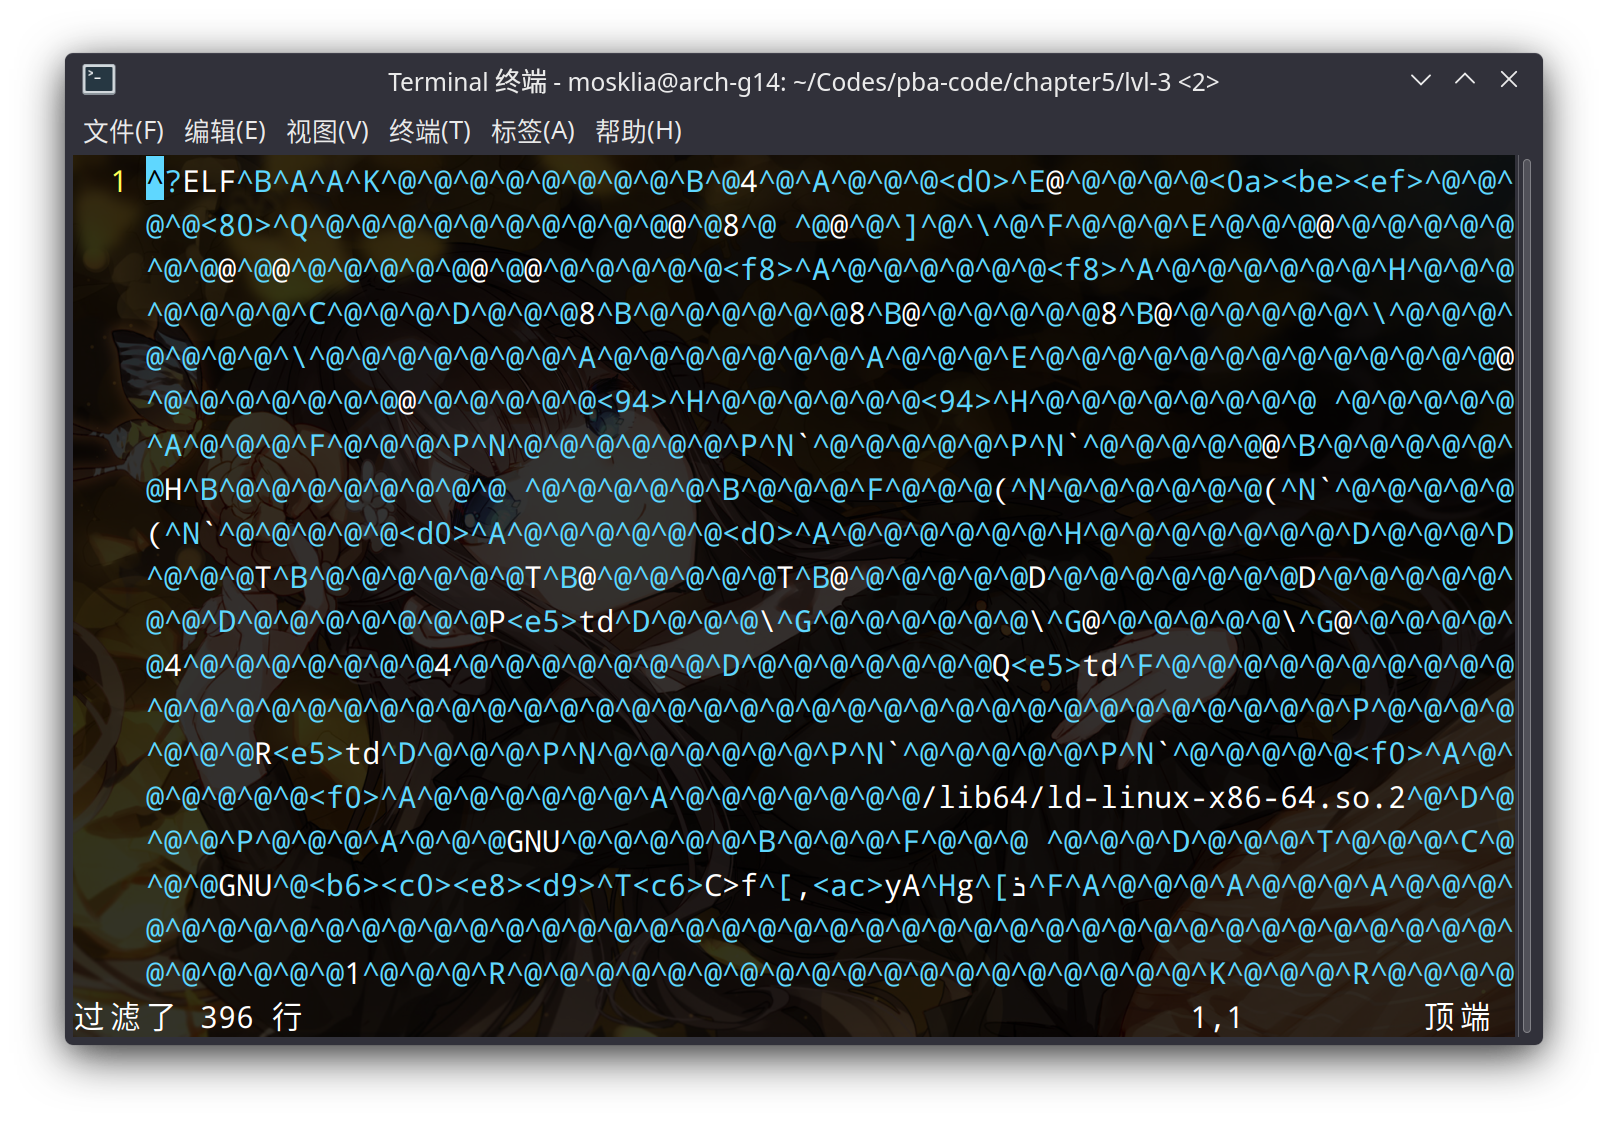
\includegraphics[width=0.45\textwidth]{pics/lvl3-vim-2.png}
        \end{center}

        使用命令 \mintinline{vim}{:%!xxd -r} 将文件重新转换为二进制文件。
    
    \end{frame}

    \begin{frame}[fragile]
    
        首先修复 OS/ABI 的错误,它是文件开头的第 8 个字节。

        将其修改为 \mintinline{text}{00}。

        \begin{center}
            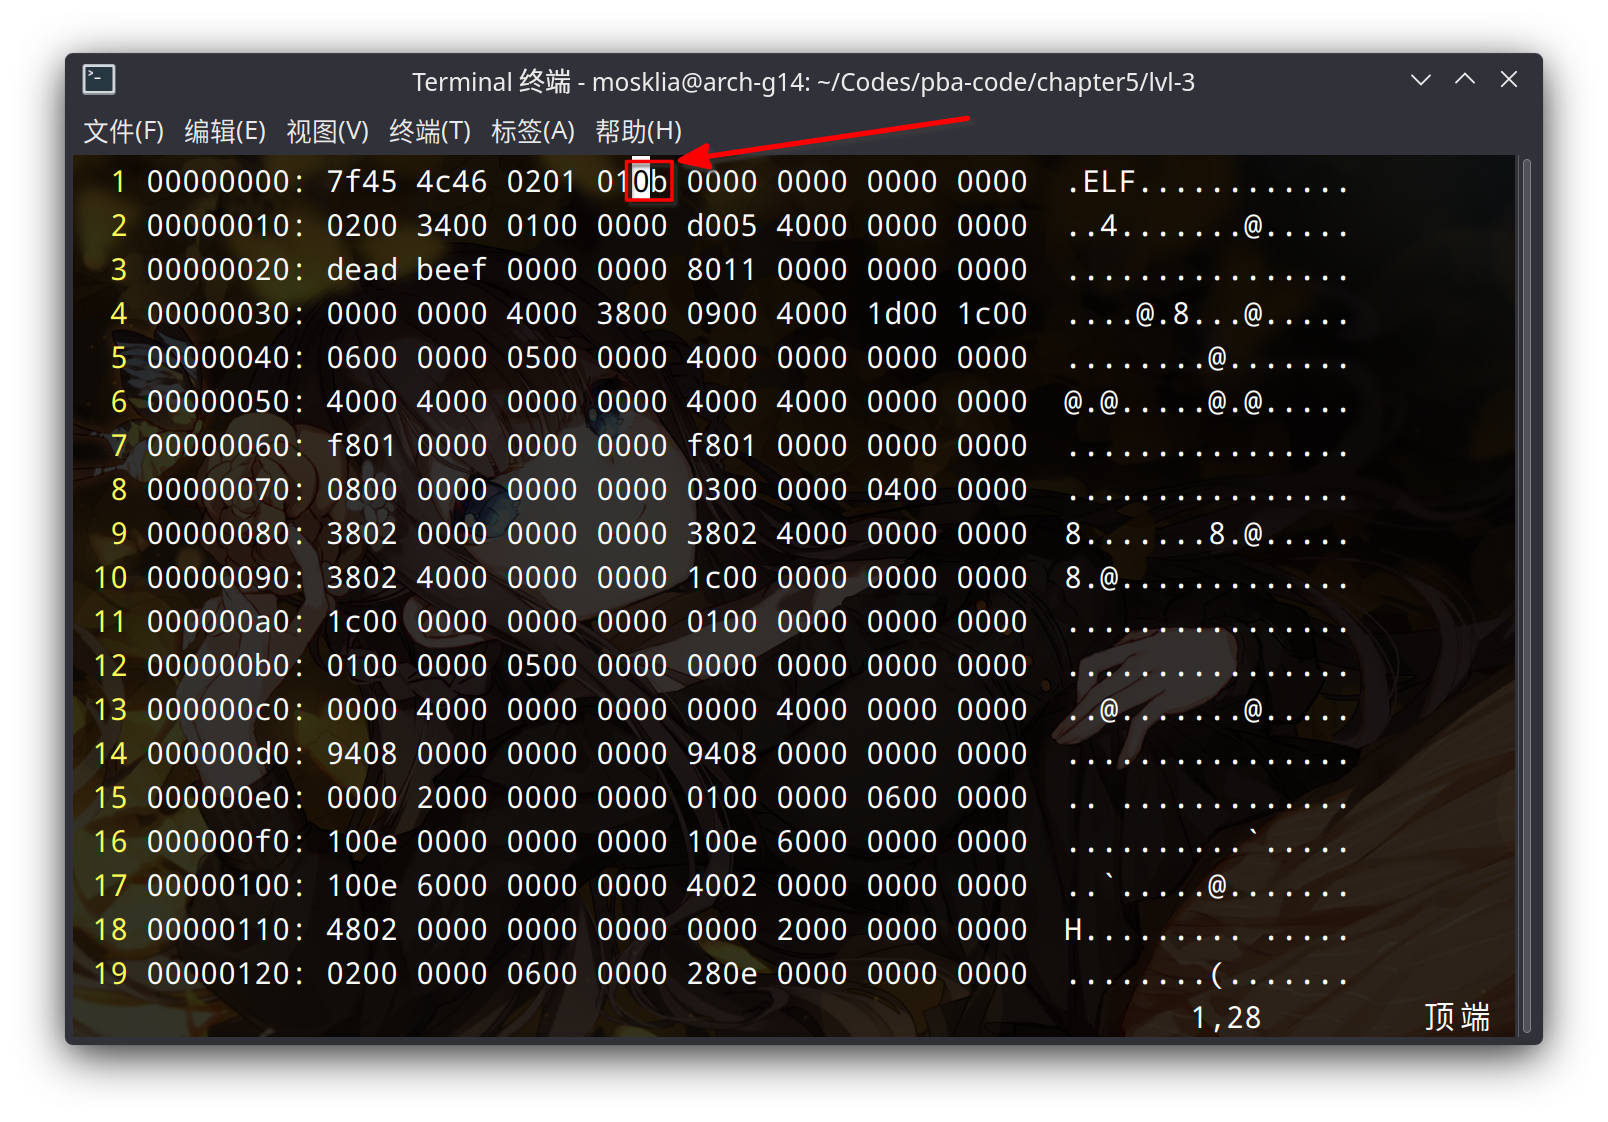
\includegraphics[width=0.45\textwidth]{pics/lvl3-error1-before.png}\;
            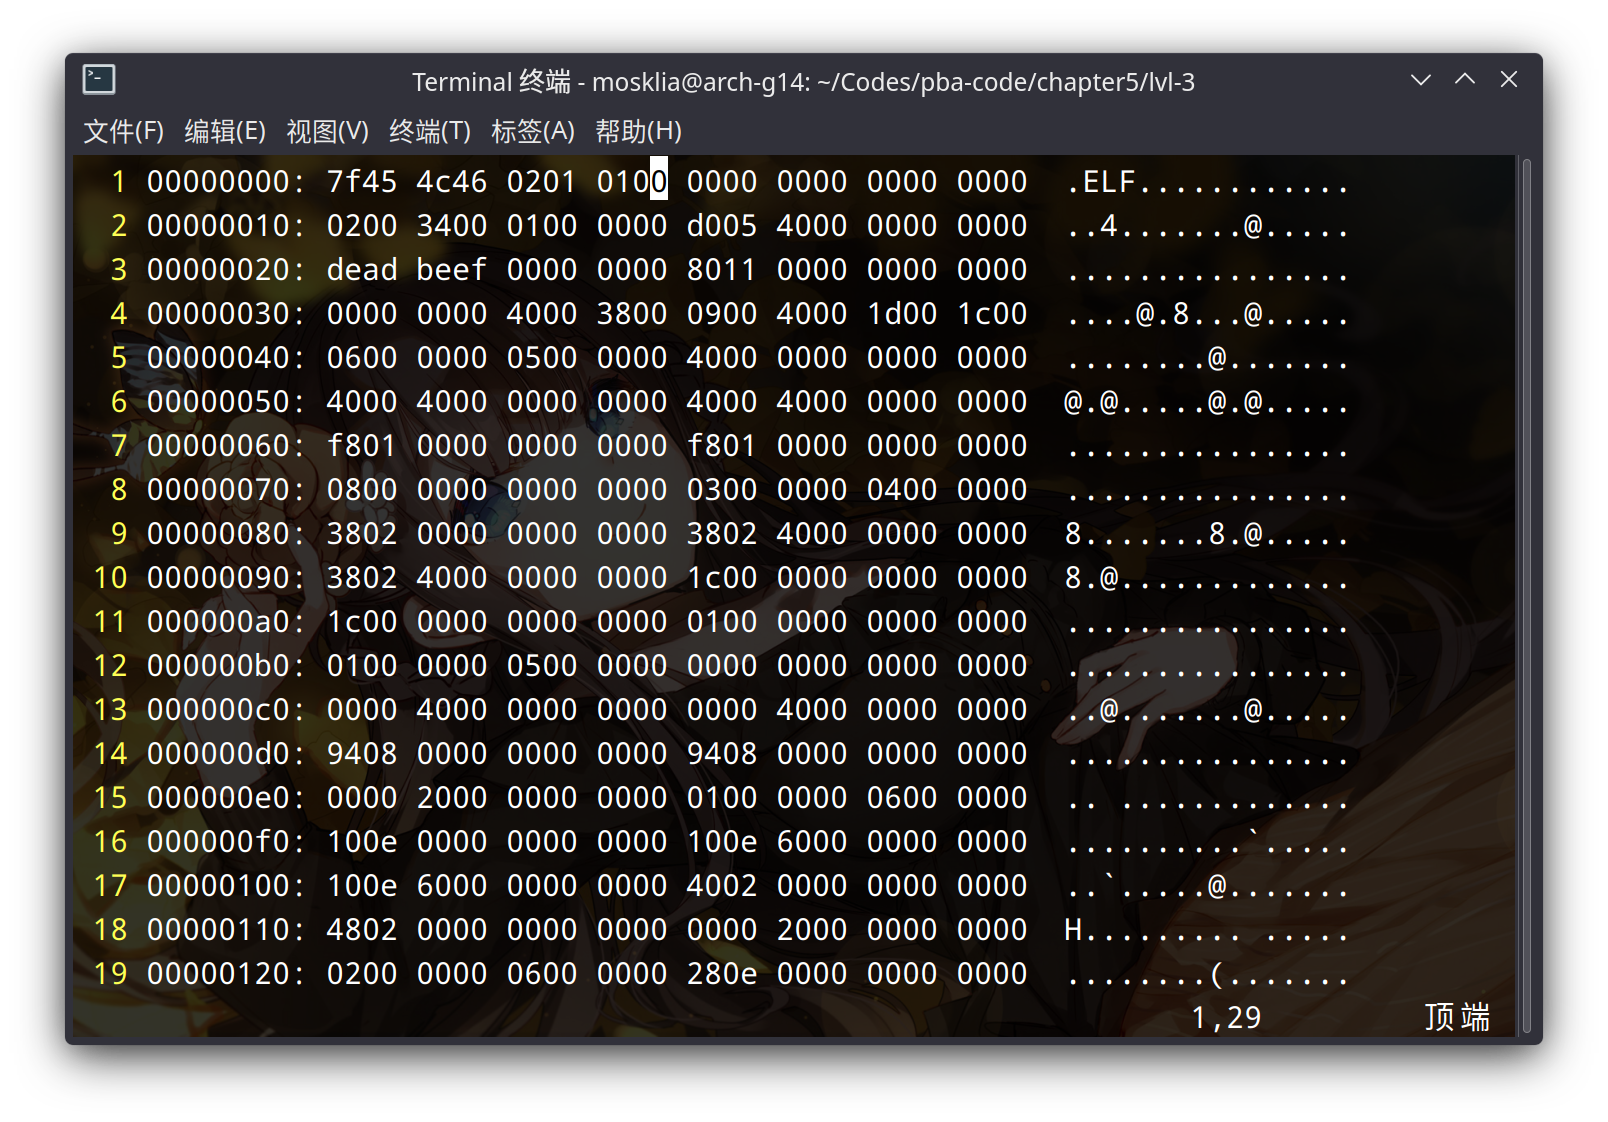
\includegraphics[width=0.45\textwidth]{pics/lvl3-error1-after.png}
        \end{center}
    
    \end{frame}

    \begin{frame}[fragile]
    
        然后修复系统架构的错误,它是文件开头的第 19 到 20 个字节。

        通过观察其他可执行文件的对应位置,可知此处应为 \mintinline{text}{3e00}。

        \begin{center}
            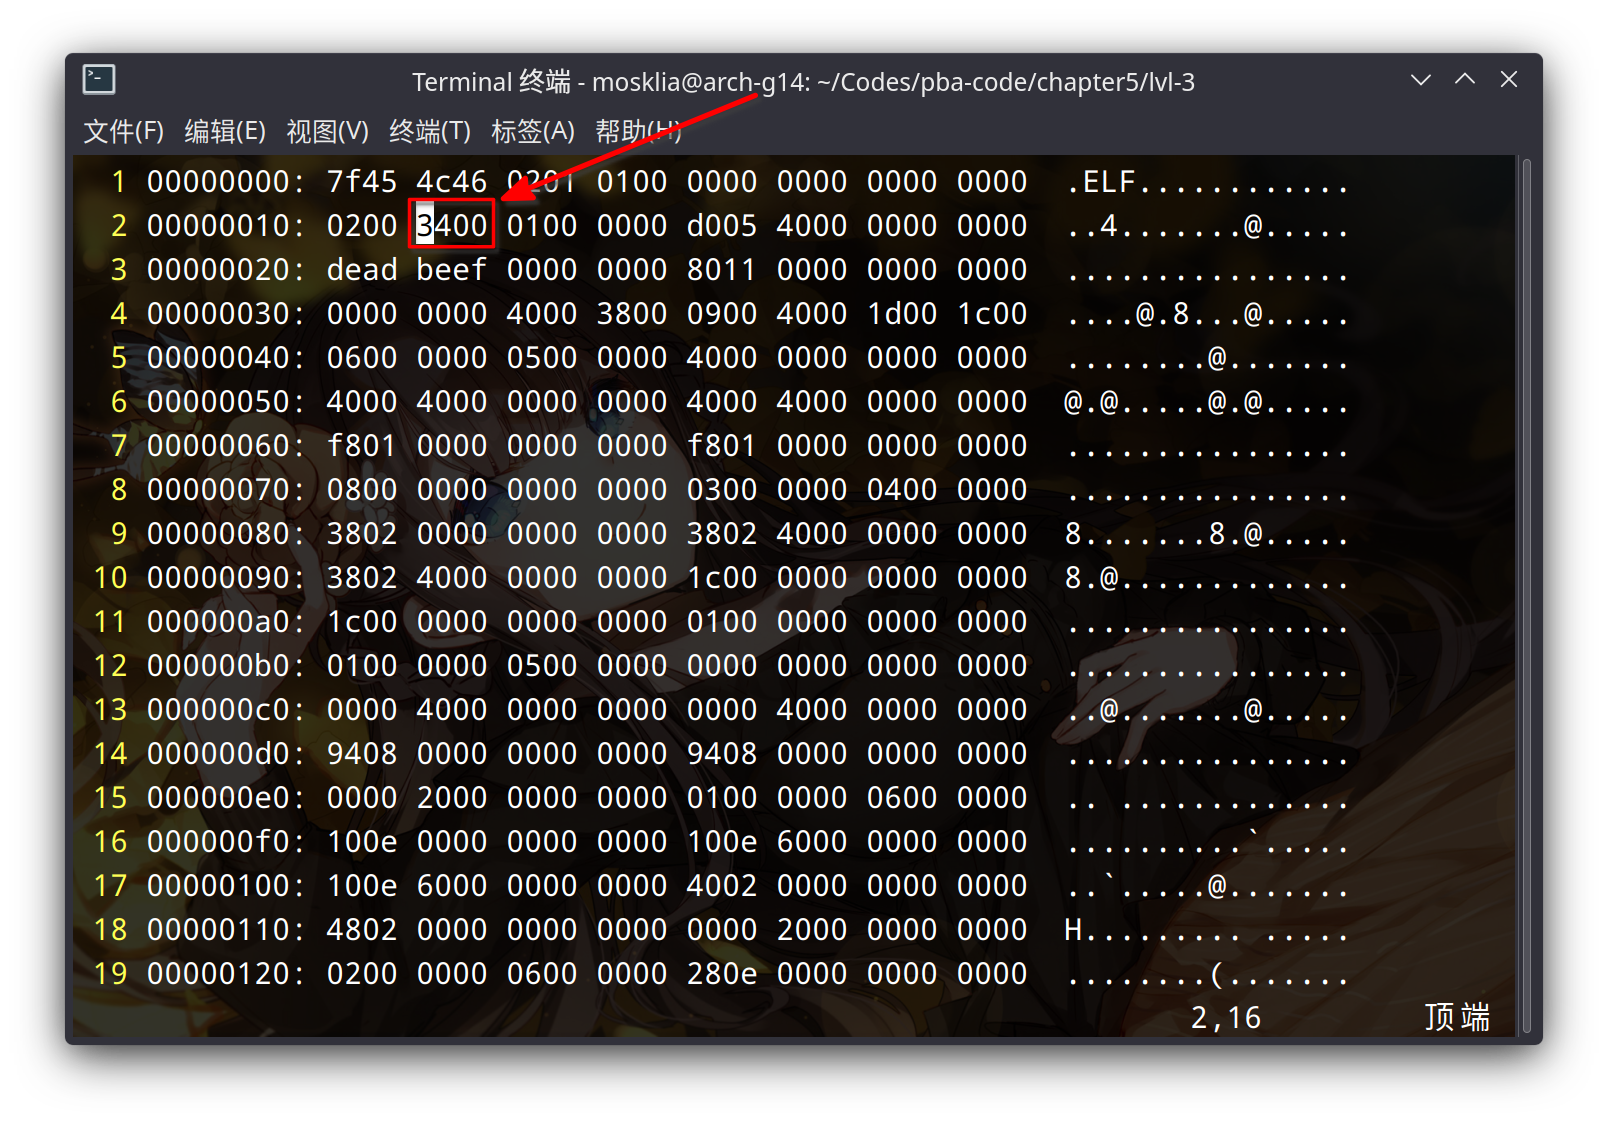
\includegraphics[width=0.45\textwidth]{pics/lvl3-error2-before.png}\;
            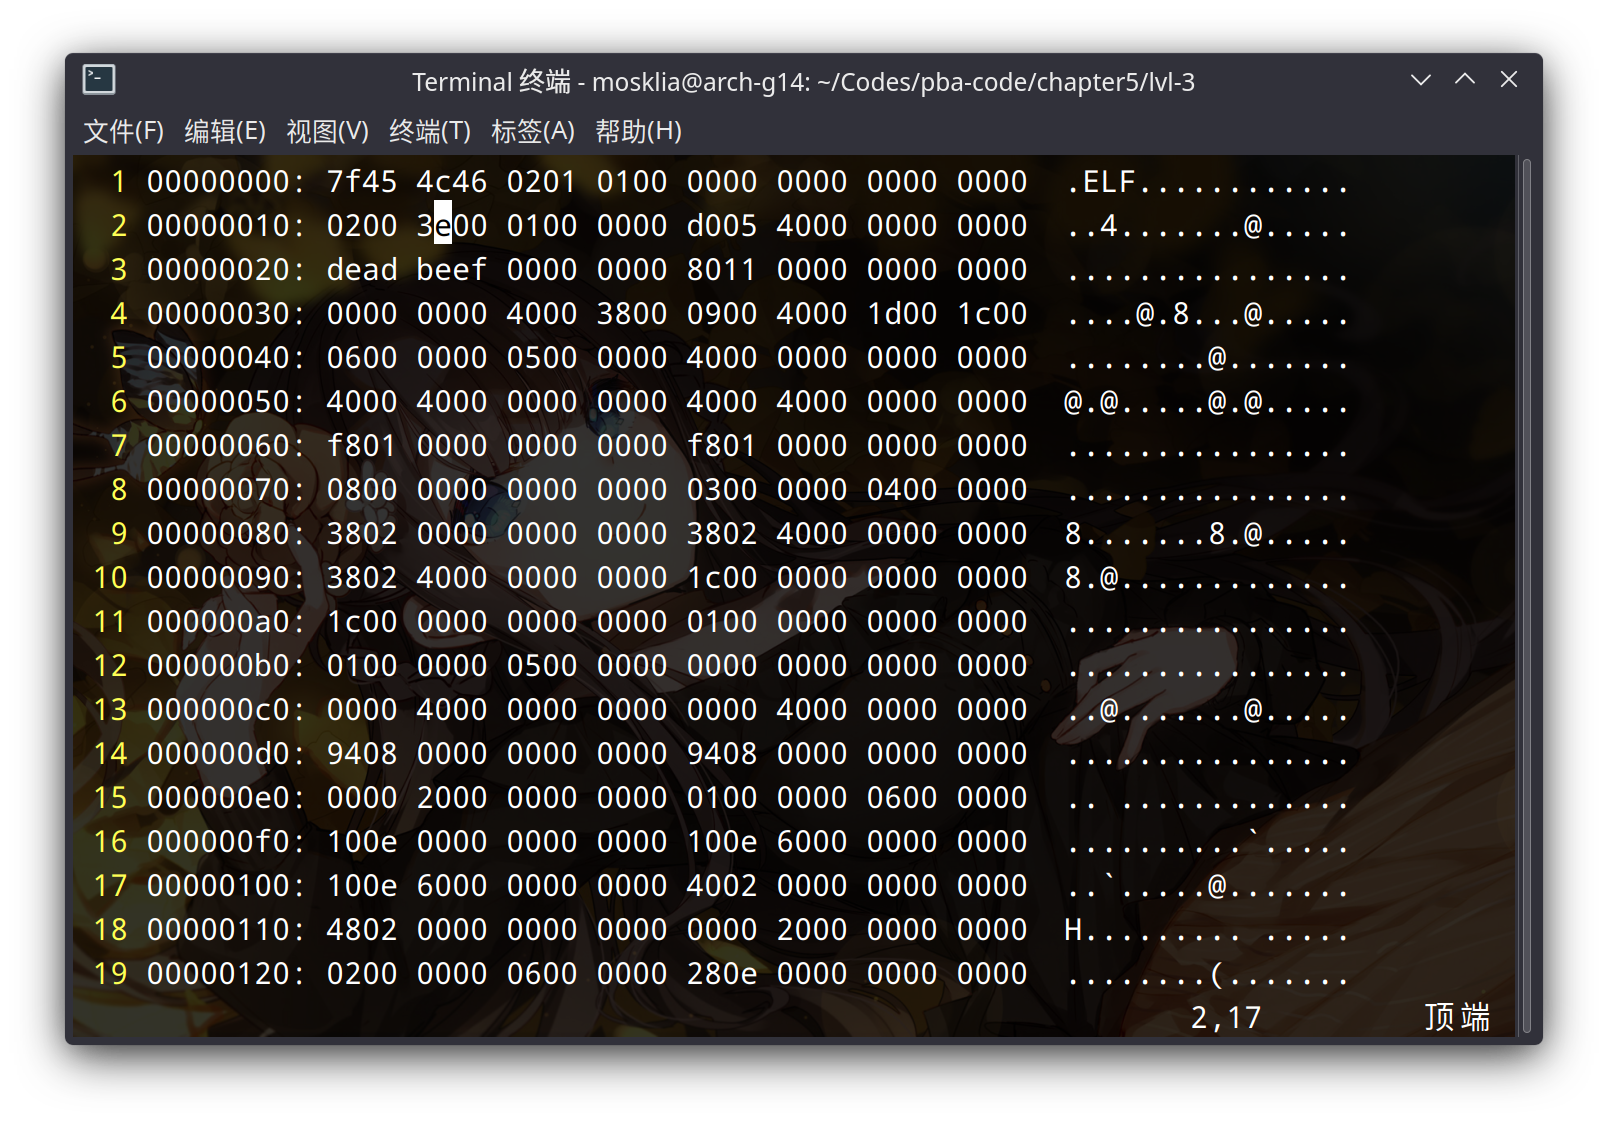
\includegraphics[width=0.45\textwidth]{pics/lvl3-error2-after.png}
        \end{center}
    
    \end{frame}

    \begin{frame}[fragile]
    
        然后修复第三处错误,也就是
        
        \begin{minted}{text}
            readelf:错误:Reading 504 bytes extends past end of file for 程序头
        \end{minted}

        的问题。 \pause

        我们知道 ELF 文件的程序头往往会紧跟在 EFL 头后面,因此我们尝试修复 \mintinline{text}{e_phoff} 的值,令其等于 ELF 头的大小。\pause
        
        那么 ELF 头的大小又是多少呢?\mintinline{zsh}{file} 命令已经告诉了我们:

        \begin{minted}{text}
            Size of this header:               64 (bytes)
        \end{minted}
    
    \end{frame}

    \begin{frame}
    
        于是将 \mintinline{text}{e_phoff},即文件的 0X20 到 0X27 字节修改为 \mintinline{text}{4000 0000}。

        \begin{center}
            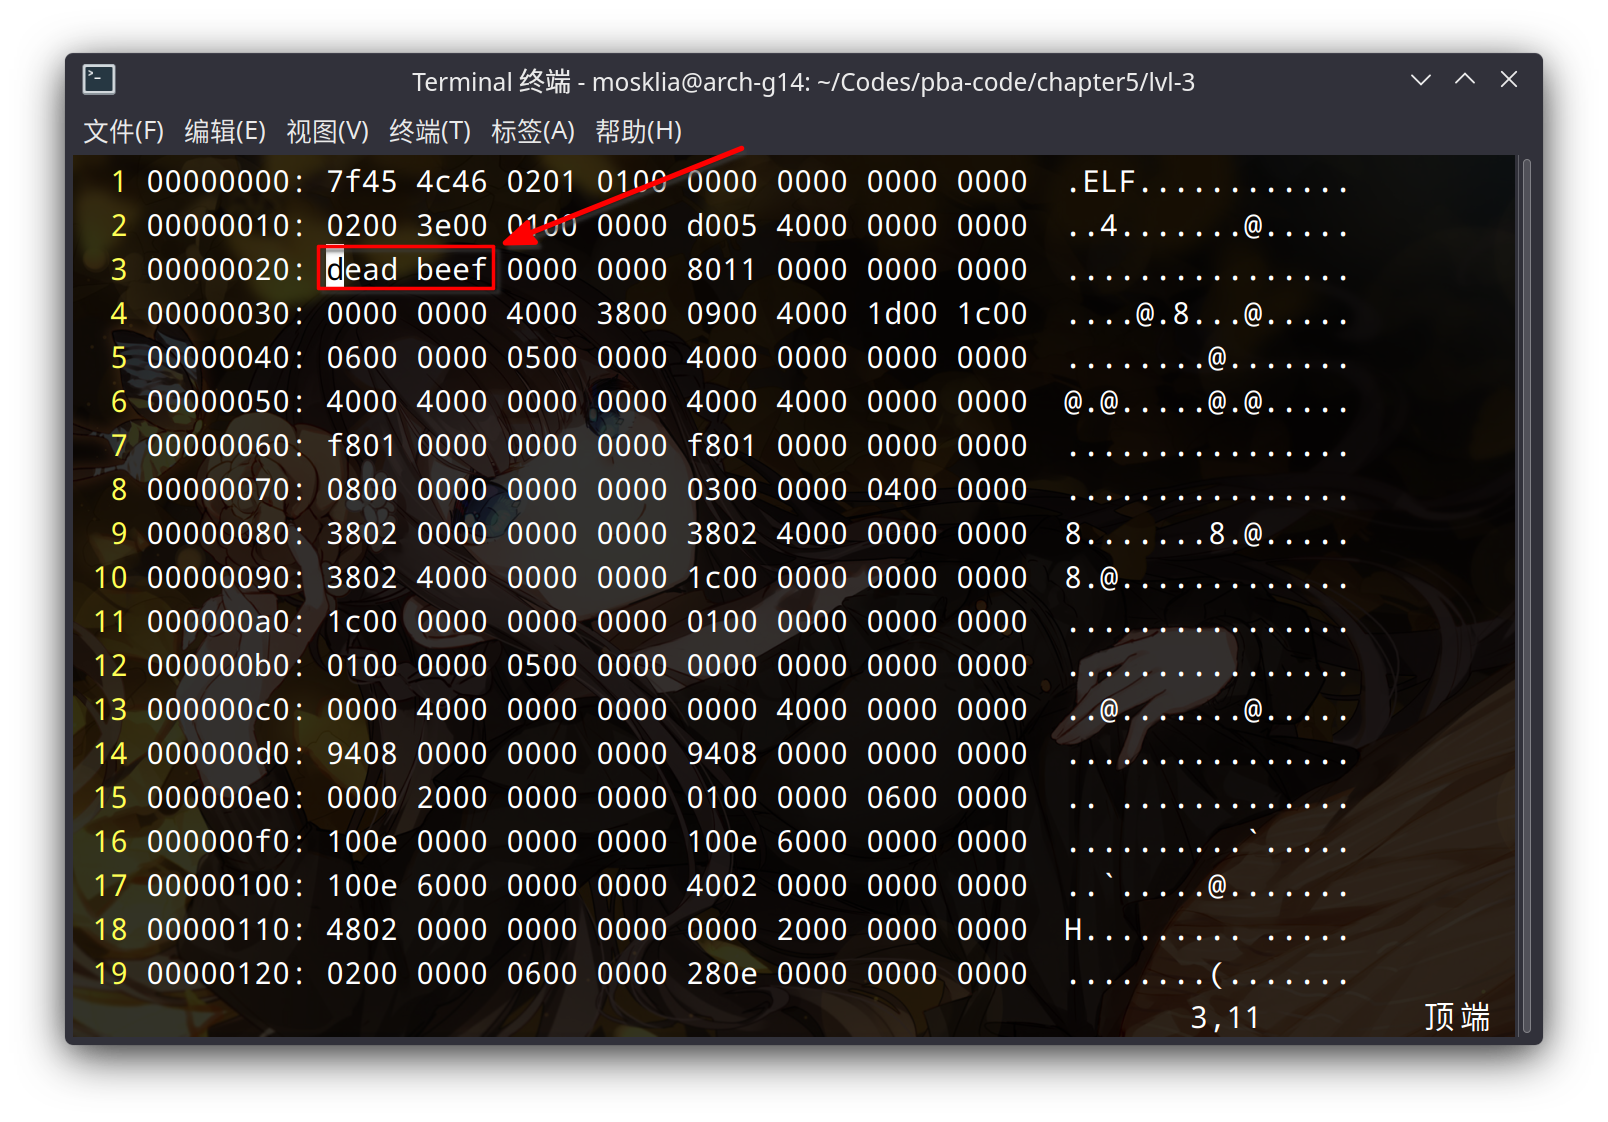
\includegraphics[width=0.45\textwidth]{pics/lvl3-error3-before.png}\;
            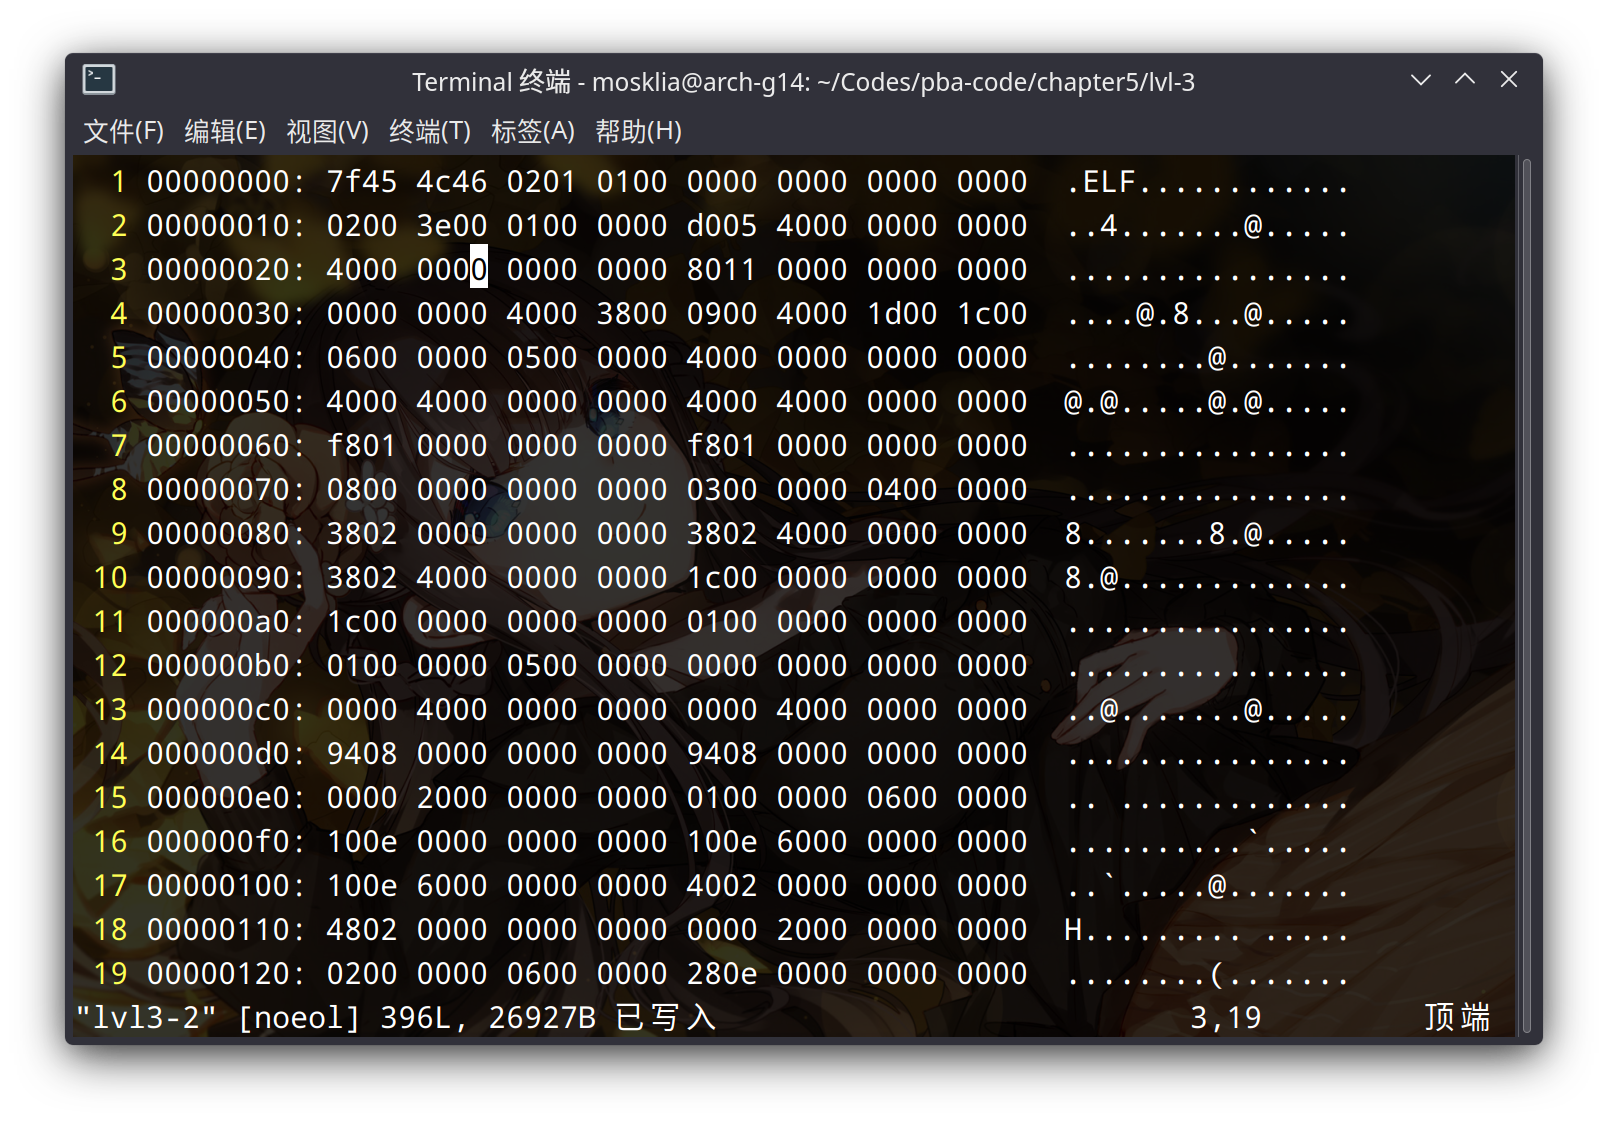
\includegraphics[width=0.45\textwidth]{pics/lvl3-error3-after.png}
        \end{center}

    \end{frame}

    \begin{frame}
    
        现在再次运行 \mintinline{zsh}{readelf -h lvl3},一切都正常了。

        \begin{center}
            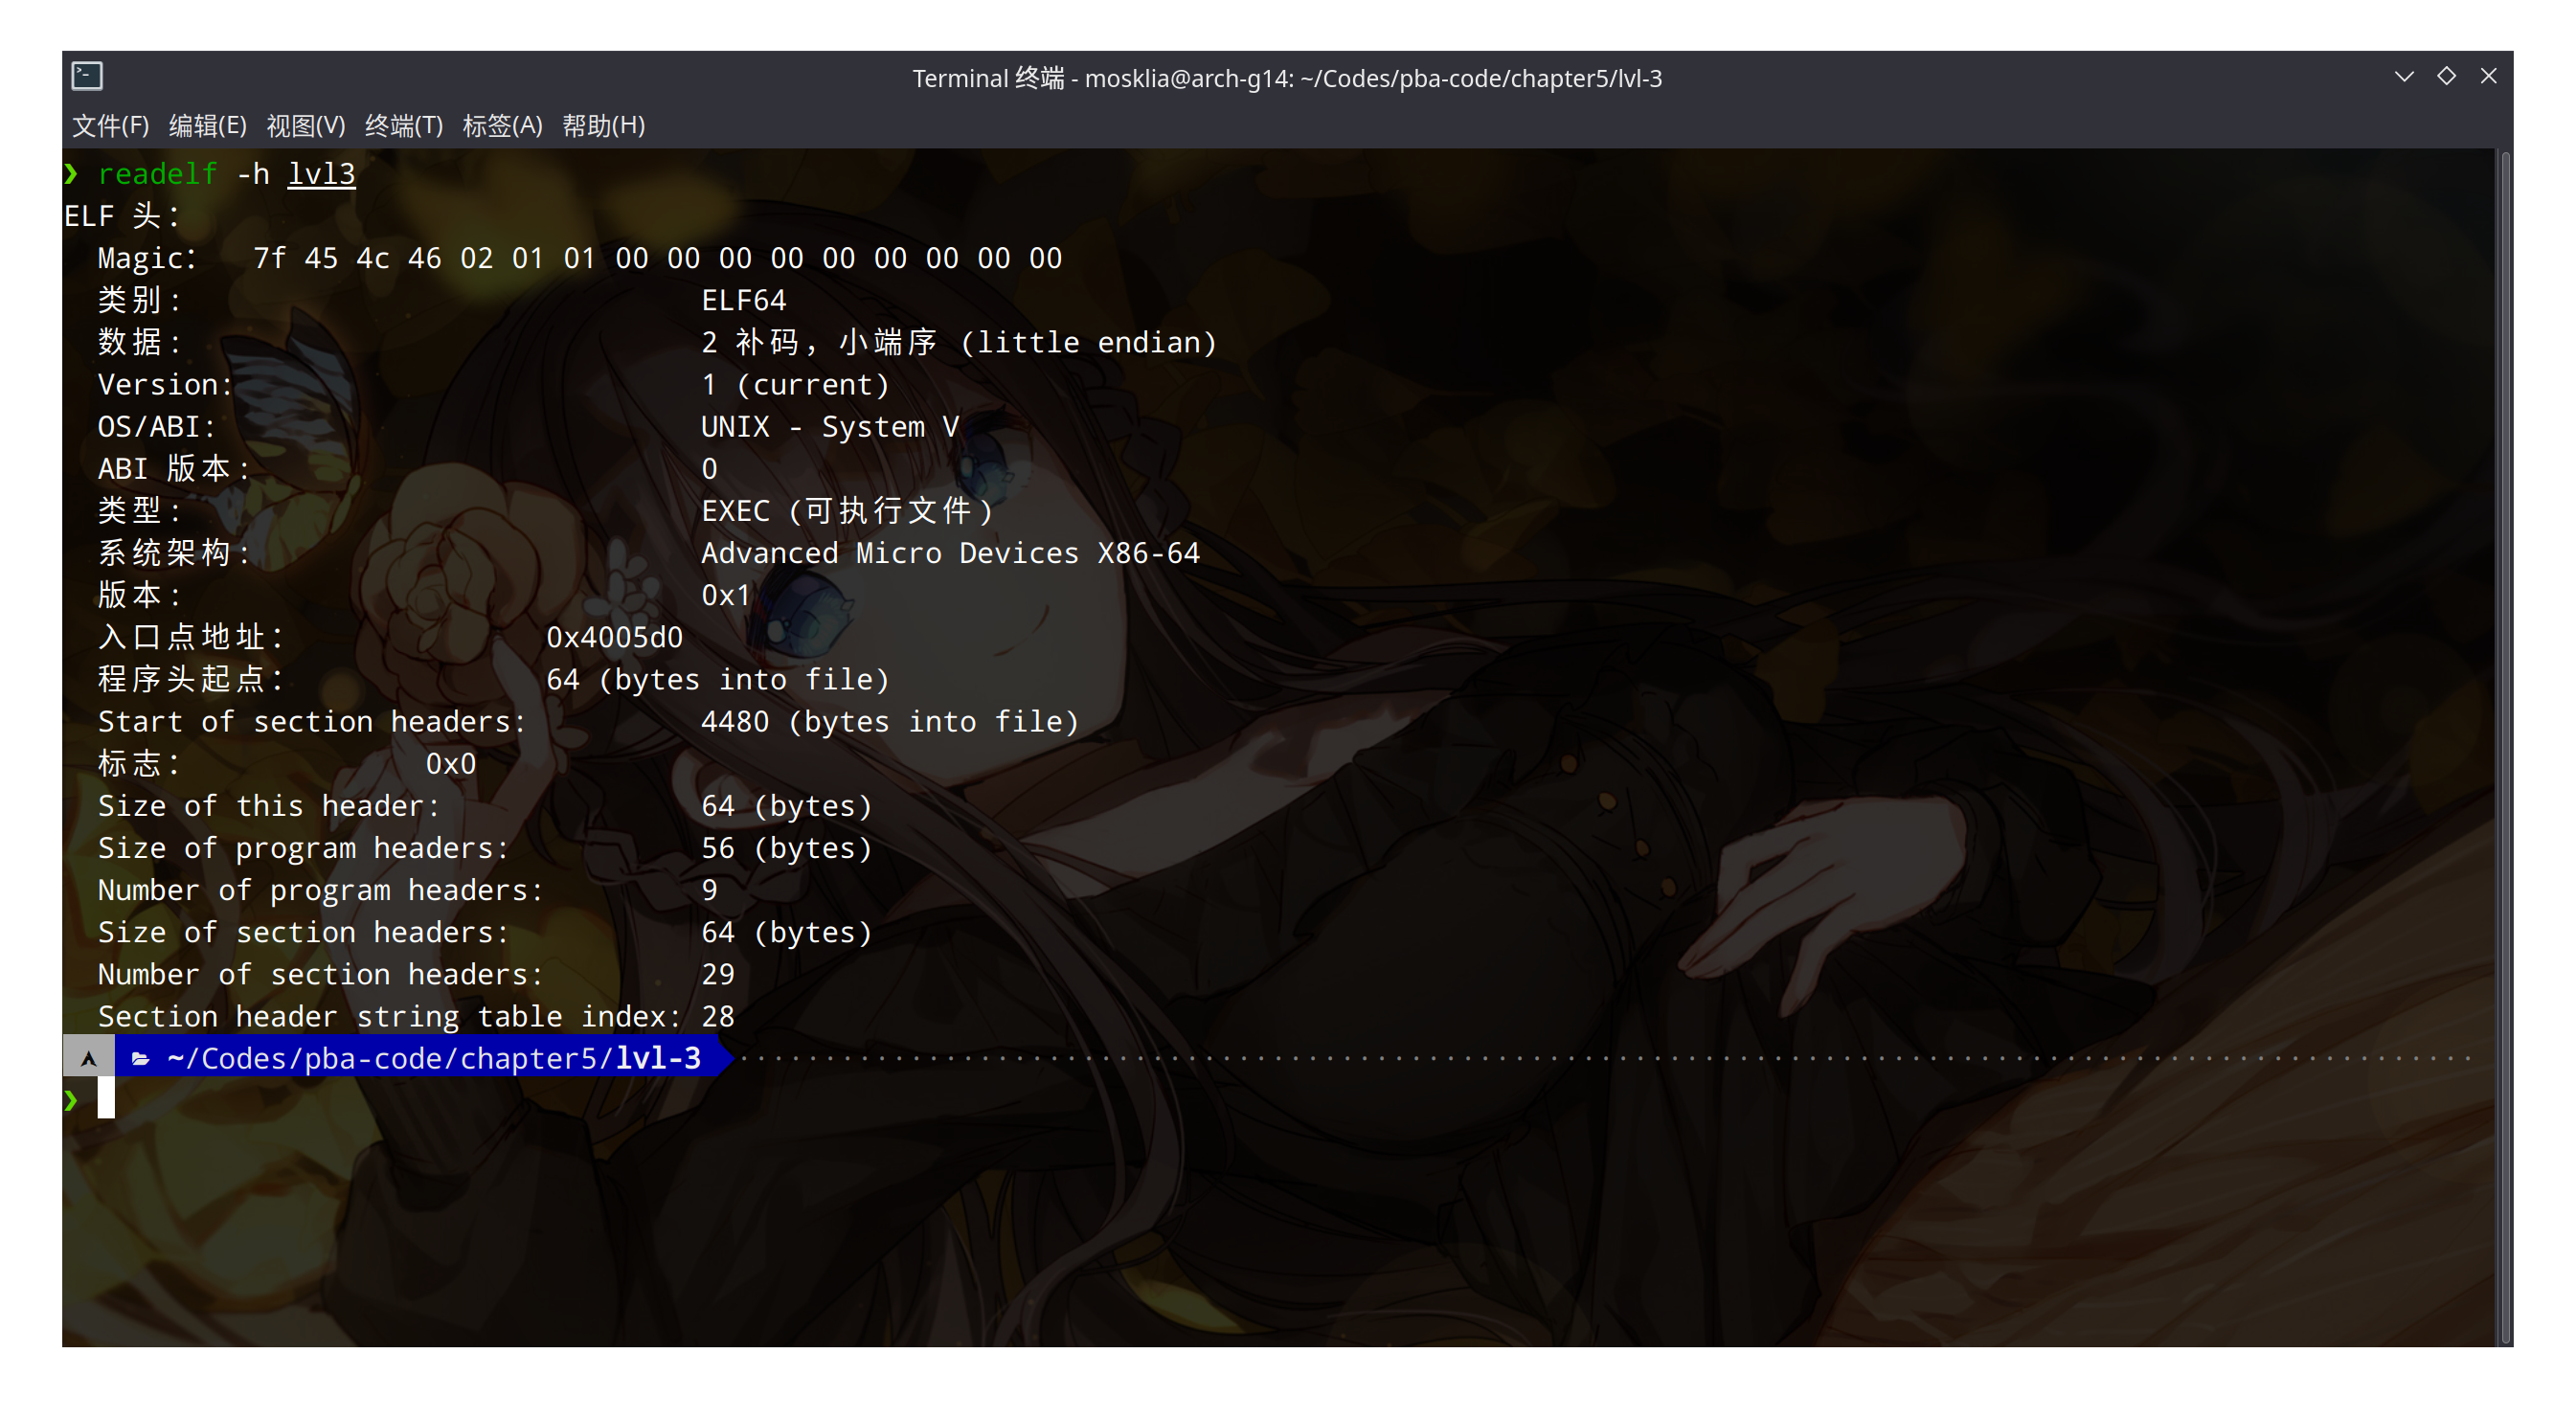
\includegraphics[width=0.9\textwidth]{pics/lvl3-readelf-stage2.png}
        \end{center}

        开香槟!(bushi)
    
    \end{frame}

    \begin{frame}[fragile]
    
        并且此时运行 \mintinline{text}{./lvl3},会得到一个输出:

        \begin{minted}{text}
            0e2ada7381d04d4d2ed31be82b121aa3  ./lvl3
        \end{minted}

        看起来很像是一个 flag。于是尝试把它提交给 oracle。\pause

        \begin{minted}{text}
            Invalid flag: 0e2ada7381d04d4d2ed31be82b121aa3
        \end{minted}

        依稀回想起来,oracle 说有四处问题,但我们只找到了三处...
    
    \end{frame}

    \begin{frame}[fragile]
        \frametitle{Level 3}
        \framesubtitle{第四处错误}
    
        看看程序逻辑?

        使用命令 \mintinline{zsh}{objdump -d -M intel --section .text lvl3},却发现输出里面什么都没有??

        \begin{minted}{text}
lvl3:     文件格式 elf64-x86-64

Disassembly of section .text:

0000000000400550 <.text>:
	    ...
        \end{minted}

        那刚刚运行的输出是怎么回事?
    
    \end{frame}

    \begin{frame}[fragile]
    
        检查一下各个节的情况。

        使用命令 \mintinline{zsh}{readelf --sections --wide lvl3},得到输出:

        \begin{minted}[highlightlines={8}]{text}
There are 29 section headers, starting at offset 0x1180:

节头:
  [Nr] Name              Type            Address          Off    Size   ES Flg Lk Inf Al
  [ 0]                   NULL            0000000000000000 000000 000000 00      0   0  0
  [ 1] .interp           PROGBITS        0000000000400238 000238 00001c 00   A  0   0  1
    ......
  [14] .text             NOBITS          0000000000400550 000550 0001f2 00  AX  0   0 16
    ......
        \end{minted}

        \pause \mintinline{text}{.text} 节的类型是 \mintinline{text}{NOBITS},也就是``不存在于可执行文件中,运行时由操作系统向其中填充 0''!

    \end{frame}

    \begin{frame}[fragile]
    
        这应该就是要找的第四处问题了。

        要修复这个问题,我们首先需要找到 \mintinline{text}{.text} 节的记录在节头表中的位置。\pause

        \mintinline{zsh}{readelf} 已经告诉我们,节头表的偏移量是 4480 字节,并且每个节头记录的大小是 64 字节,以及 \mintinline{text}{.text} 节的序号是 14。于是可以算出,这个记录的偏移量是:

        \begin{align*}
            offset &= e\_shoff + Nr \times e\_shentsize \\
            &= 4480 + 14 \times 64 \\
            &= 5376 \\
            &= \mathrm{1500_{(16)}}
        \end{align*}

        即这个记录在文件中的位置为 0X1500 到 0X153F。
    
    \end{frame}

    \begin{frame}[fragile]
    
        我们知道在节头中,节类型所在的位置是第 3 到 4 个字节。

        通过观察其他可执行文件的对应位置,可以知道这个字段的值(\mintinline{text}{SHT_PROGBITS})应为 \mintinline{text}{0100 0000}。

        \begin{center}
            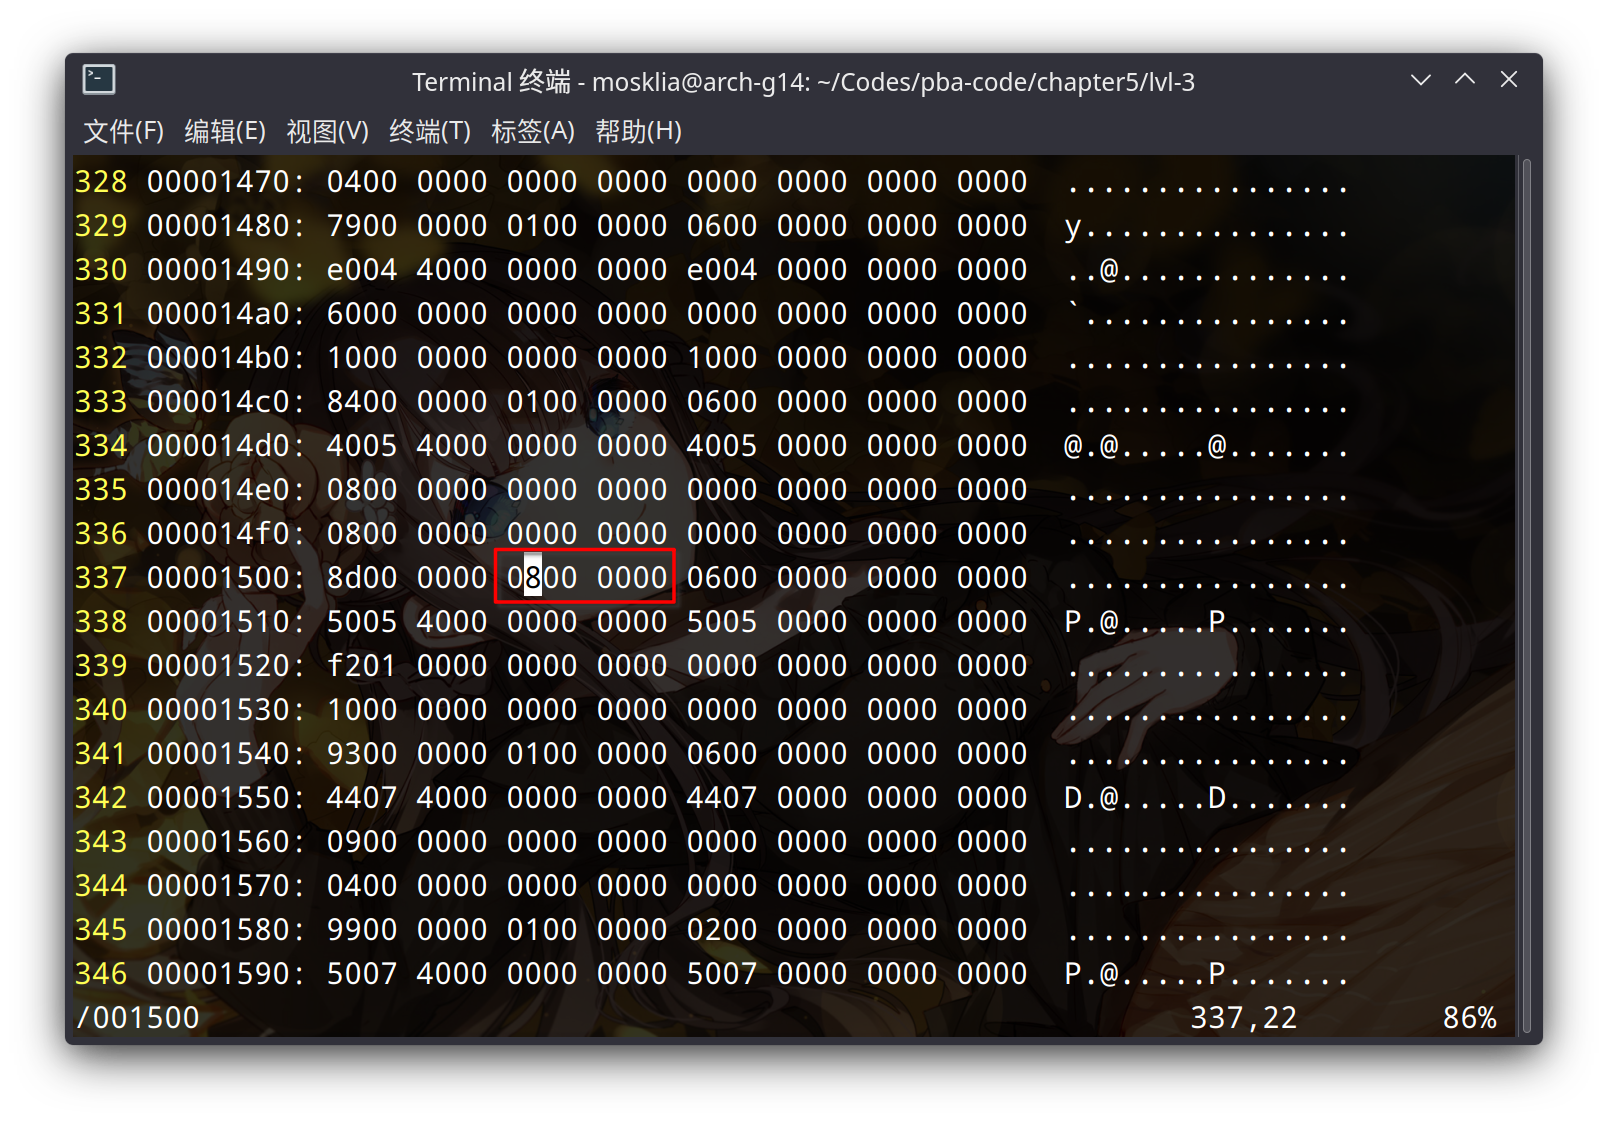
\includegraphics[width=0.45\textwidth]{pics/lvl3-error4-before.png}\;
            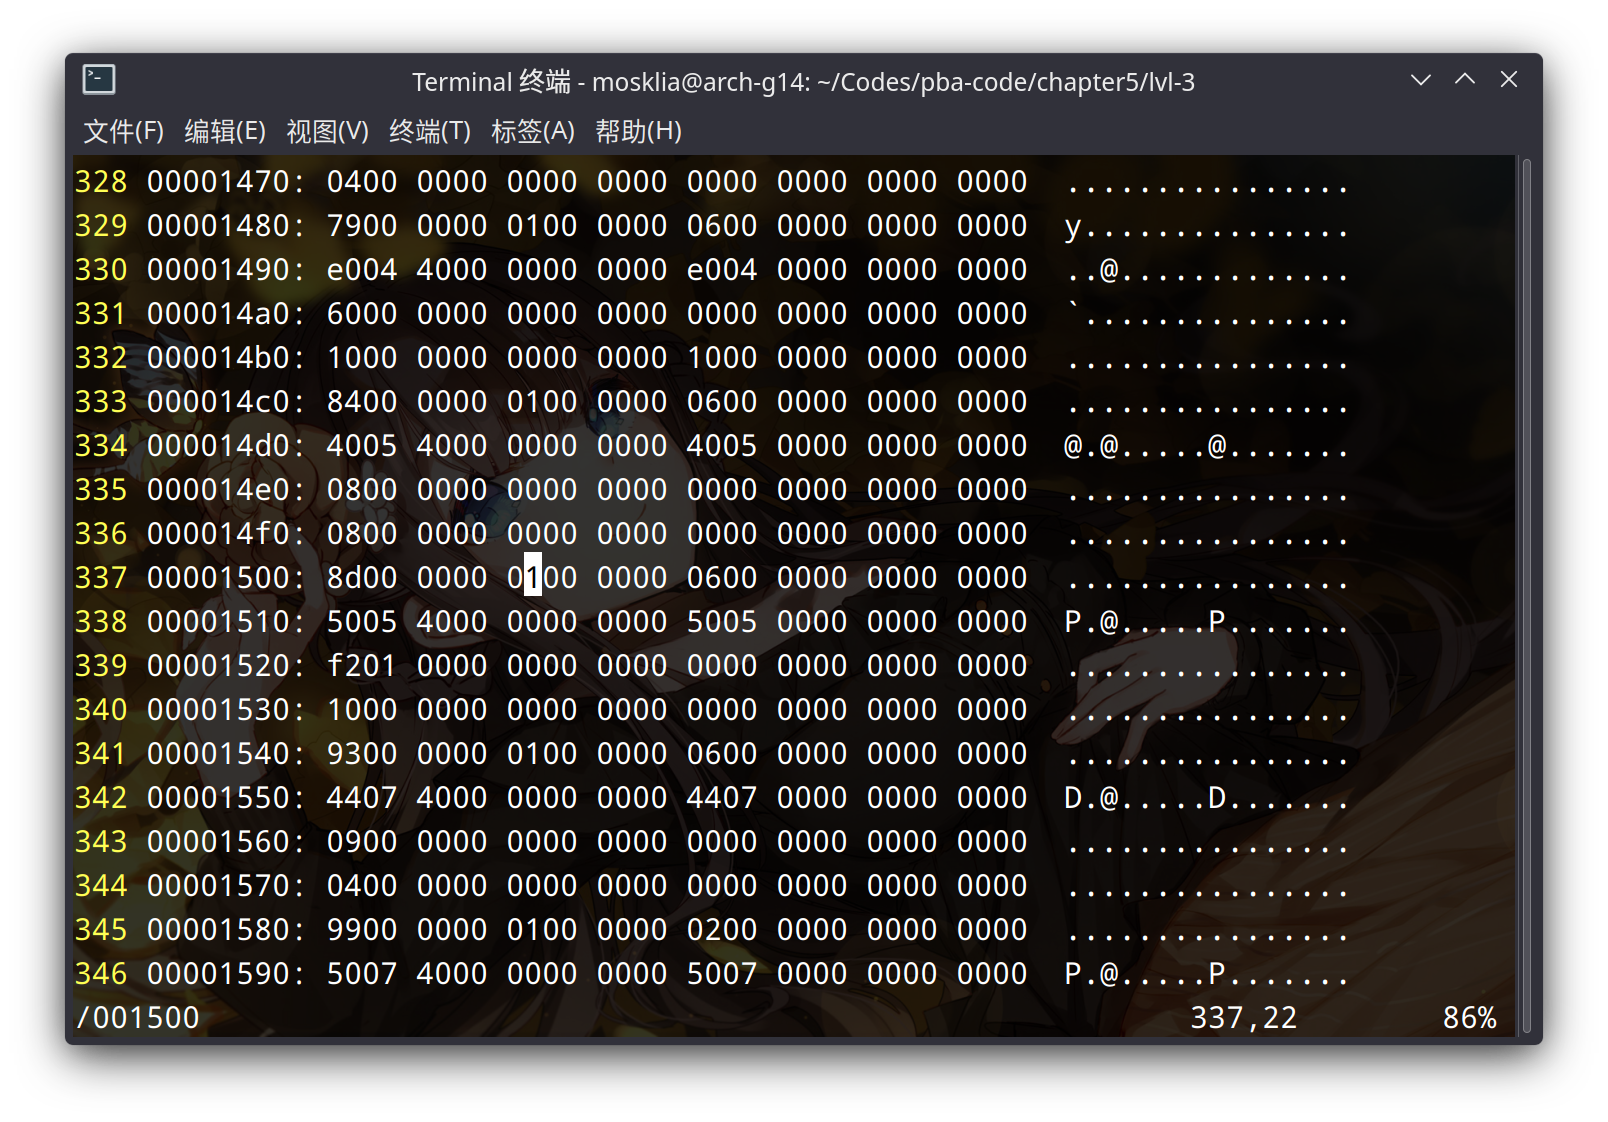
\includegraphics[width=0.45\textwidth]{pics/lvl3-error4-after.png}
        \end{center}
    
    \end{frame}

    \begin{frame}[fragile]
        \frametitle{Level 3}
        \framesubtitle{The flag}
    
        再次运行 \mintinline{zsh}{./lvl3},得到新的输出:

        \begin{minted}{text}
            3a5c381e40d2fffd95ba4452a0fb4a40  ./lvl3
        \end{minted}

        经过验证,这次的输出是正确的 flag。
    
    \end{frame}

    \section{Level 5}

    \begin{frame}[fragile]
        \frametitle{Level 5}
        \framesubtitle{提示}
    
        \mintinline{text}{oracle} 给出的提示为:

        \begin{minted}{text}
               Secrets hidden in code unused
                  秘密隐藏在未使用的代码之中
            The method of redirection is the key
                  重定位的方法就是解密的关键
               Static rather than dynamically
                     静态的,而非动态的
        \end{minted}

        看来,一次反汇编是必不可少的了。
    
    \end{frame}

    \begin{frame}[fragile]
        \frametitle{Level 5}
        \framesubtitle{直接运行}
    
        直接运行程序,得到输出结果:

        \begin{minted}{text}
            nothing to see here
        \end{minted}

        且程序返回了 1。
    
    \end{frame}

    \begin{frame}[fragile]
        \frametitle{Level 5}
        \framesubtitle{反汇编}
    
        先反汇编只读数据节 \mintinline{text}{.rodata}:

        {
            \small
            \begin{minted}{text}
                Contents of section .rodata:
                 400770 01000200 6b657920 3d203078 25303878  ....key = 0x%08x
                 400780 0a006465 63727970 74656420 666c6167  ..decrypted flag
                 400790 203d2025 730a006e 6f746869 6e672074   = %s..nothing t
                 4007a0 6f207365 65206865 726500             o see here.     
            \end{minted}
        }


        \pause
        可以看到几个有趣的字符串:\pause

        \begin{enumerate}
            \item \mintinline{text}{key = 0x%08x},位于 0X400774 处;\pause
            \item \mintinline{text}{descrypted flag = %s},位于 0X400782 处; \pause
            \item \mintinline{text}{nothing to see here},刚刚直接运行时输出的内容,位于 0X400797 处。
        \end{enumerate}
    
    \end{frame}

    \begin{frame}[fragile]
    
        这时再回去看代码。反汇编代码节 \mintinline{text}{.text}:

        {
            \small
            \begin{minted}[highlightlines={3,7}]{text}
                0000000000400500 <.text>:
                  400500:	48 83 ec 08          	sub    rsp,0x8
                  400504:	bf 97 07 40 00       	mov    edi,0x400797
                  400509:	e8 a2 ff ff ff       	call   4004b0 <puts@plt>
                  40050e:	b8 01 00 00 00       	mov    eax,0x1
                  400513:	48 83 c4 08          	add    rsp,0x8
                  400517:	c3                   	ret
                  400518:	0f 1f 84 00 00 00 00 	nop    DWORD PTR [rax+rax*1+0x0]
                  ......
            \end{minted}
        }

        居然直接返回了,下面一大段代码都没用上。\pause

        说明下面的代码里面一定有猫腻!
    
    \end{frame}

    \begin{frame}[fragile]
    
        于是将重点放在涉及两个地址,0X400774 和 0X400782,以及有输出调用的代码处。\pause

        {
            \small
            \begin{minted}{text}
                400620:	53                   	push   rbx
                400621:	be 74 07 40 00       	mov    esi,0x400774
                ......
                40068a:	e8 51 fe ff ff       	call   4004e0 <__printf_chk@plt>
                ......
                4006ab:	31 c0                	xor    eax,eax
                4006ad:	48 89 e2             	mov    rdx,rsp
                4006b0:	be 82 07 40 00       	mov    esi,0x400782
                4006b5:	bf 01 00 00 00       	mov    edi,0x1
                4006ba:	e8 21 fe ff ff       	call   4004e0 <__printf_chk@plt>
            \end{minted}
            \pause
        }

        这范围内有一大片代码,看起来很有趣...
    
    \end{frame}

    \begin{frame}[fragile]

        0X400774:
    
        {
            \tiny
            \begin{minted}{text}
                400620:	53                   	push   rbx
                400621:	be 74 07 40 00       	mov    esi,0x400774
                400626:	bf 01 00 00 00       	mov    edi,0x1
                40062b:	48 83 ec 30          	sub    rsp,0x30
                40062f:	64 48 8b 04 25 28 00 	mov    rax,QWORD PTR fs:0x28
                400636:	00 00 
                400638:	48 89 44 24 28       	mov    QWORD PTR [rsp+0x28],rax
                40063d:	31 c0                	xor    eax,eax
                40063f:	48 b8 10 60 21 33 15 	movabs rax,0x6223331533216010
                400646:	33 23 62 
                400649:	c6 44 24 20 00       	mov    BYTE PTR [rsp+0x20],0x0
                40064e:	48 89 04 24          	mov    QWORD PTR [rsp],rax
                400652:	48 b8 45 65 76 34 41 	movabs rax,0x6675364134766545
                400659:	36 75 66 
                40065c:	48 89 44 24 08       	mov    QWORD PTR [rsp+0x8],rax
                400661:	48 b8 17 67 75 64 10 	movabs rax,0x6570331064756717
                400668:	33 70 65 
                40066b:	48 89 44 24 10       	mov    QWORD PTR [rsp+0x10],rax
                400670:	48 b8 18 35 76 62 11 	movabs rax,0x6671671162763518
                400677:	67 71 66 
                40067a:	48 89 44 24 18       	mov    QWORD PTR [rsp+0x18],rax
                40067f:	8b 1c 25 40 05 40 00 	mov    ebx,DWORD PTR ds:0x400540
                400686:	31 c0                	xor    eax,eax
                400688:	89 da                	mov    edx,ebx
                40068a:	e8 51 fe ff ff       	call   4004e0 <__printf_chk@plt>
                40068f:	48 8d 54 24 20       	lea    rdx,[rsp+0x20]
                400694:	48 89 e0             	mov    rax,rsp
                400697:	66 0f 1f 84 00 00 00 	nop    WORD PTR [rax+rax*1+0x0]
                40069e:	00 00 
            \end{minted}
        }

        \pause 除了输出寄存器 \mintinline{text}{rbx} 的值以外,这部分代码在把一些硬编码的魔数写进栈上的空间里面。
    
    \end{frame}

    \begin{frame}[fragile]

        两者之间:
    
        {
            \scriptsize
            \begin{minted}{text}
                40068f:	48 8d 54 24 20       	lea    rdx,[rsp+0x20]
                400694:	48 89 e0             	mov    rax,rsp
                400697:	66 0f 1f 84 00 00 00 	nop    WORD PTR [rax+rax*1+0x0]
                40069e:	00 00 
                4006a0:	31 18                	xor    DWORD PTR [rax],ebx
                4006a2:	48 83 c0 04          	add    rax,0x4
                4006a6:	48 39 d0             	cmp    rax,rdx
                4006a9:	75 f5                	jne    4006a0 <__gmon_start__@plt+0x1b0>
                4006ab:	31 c0                	xor    eax,eax
                4006ad:	48 89 e2             	mov    rdx,rsp
                4006b0:	be 82 07 40 00       	mov    esi,0x400782
                4006b5:	bf 01 00 00 00       	mov    edi,0x1
                4006ba:	e8 21 fe ff ff       	call   4004e0 <__printf_chk@plt>
            \end{minted}
        }

        \pause 这一部分代码又在对刚刚写入的魔数每四字节地做着异或寄存器 \mintinline{text}{ebx} 的操作。
    
    \end{frame}

    \begin{frame}[fragile]
        \frametitle{Level 5}
        \framesubtitle{使用 GDB}
    
        加上之前的种种迹象,我们可以确定,我们有必要尝试从 0X400620 开始运行程序,看看能得到什么。

        GDB 的 jump 命令可以轻松完成这个任务。\pause

        \begin{center}
            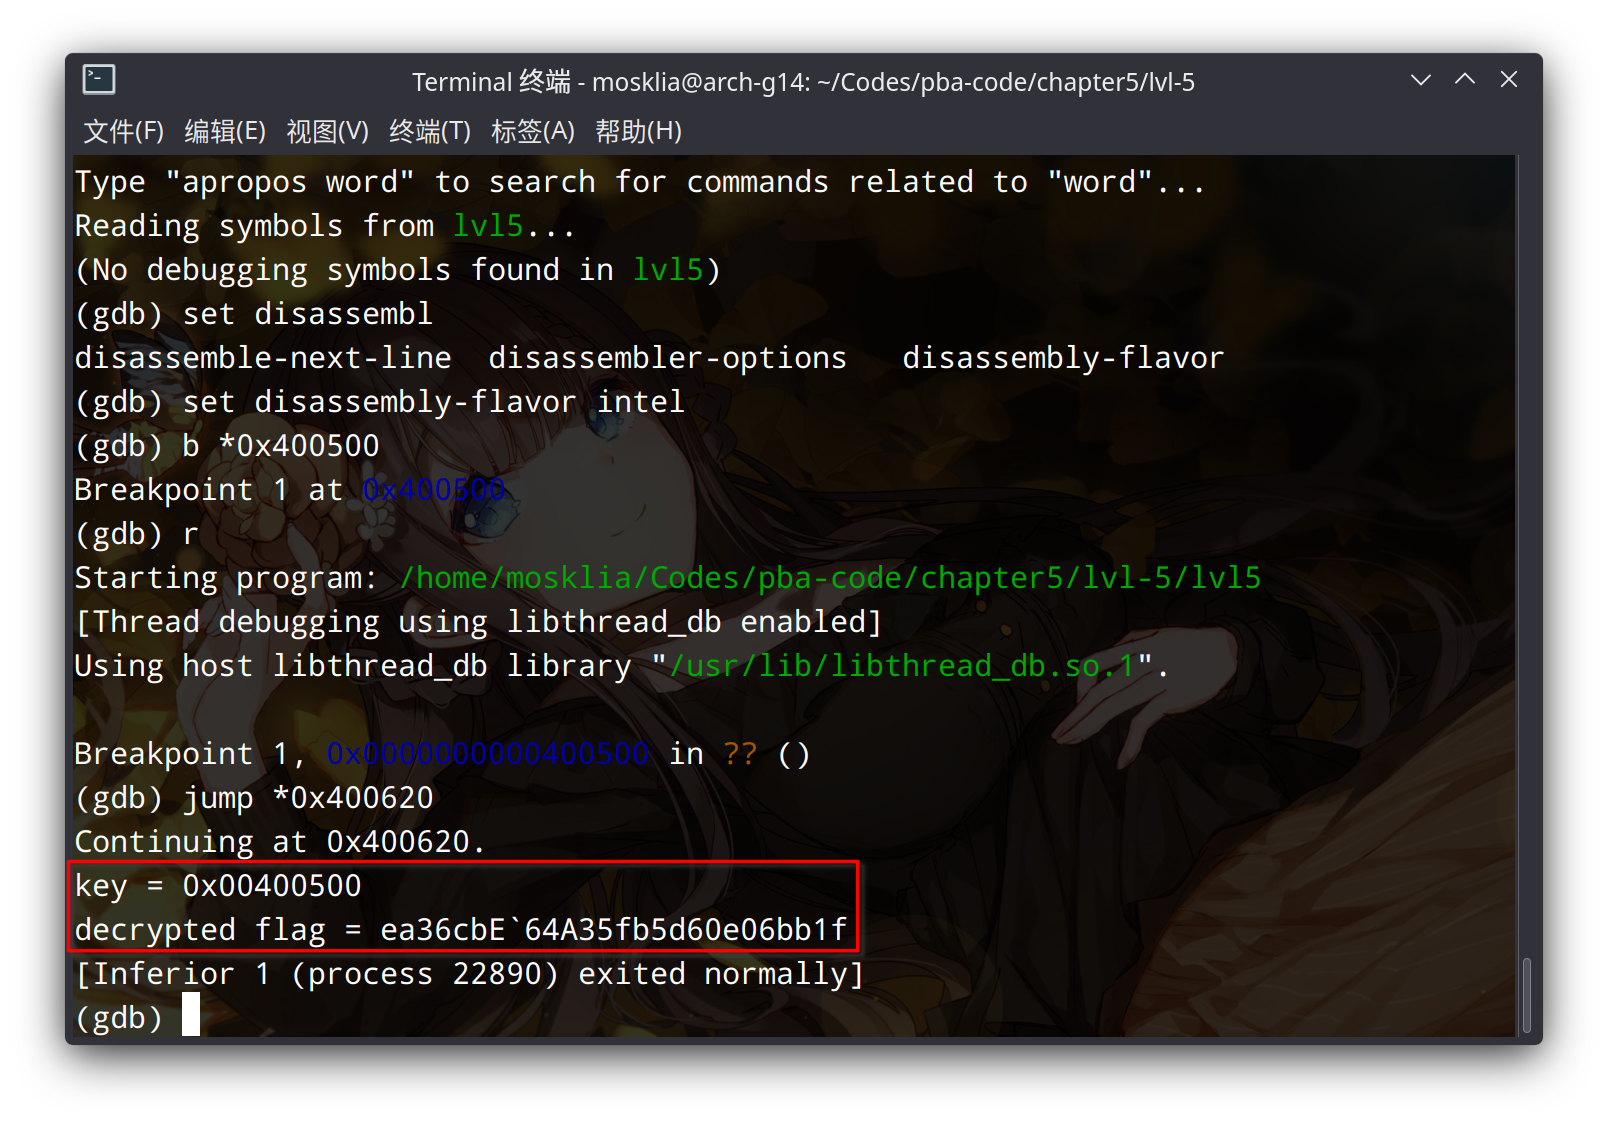
\includegraphics[width=0.5\textwidth]{pics/lvl5-gdb-1.png}
        \end{center}

        可以看到程序正常退出,并且输出了一个 flag。但是这个 flag 包含一个 \mintinline{text}{`},很明显不是合法的 flag。
    
    \end{frame}

    \begin{frame}
        \frametitle{Lvevl 5}
        \framesubtitle{Capture the Flag}
    
        看着输出中的 \mintinline{text}{key},再联系提示中说到,``重定位的方法就是解密的关键'',我们猜测:重定位的地址 0X400620 会不会就是 \mintinline{text}{key} 的正确值?

        于是再次运行 GDB, 并在给 \mintinline{text}{key}(即寄存器 \mintinline{text}{rbx})赋值的位置后面加上一个断点,修改其值并继续运行:

        \begin{center}
            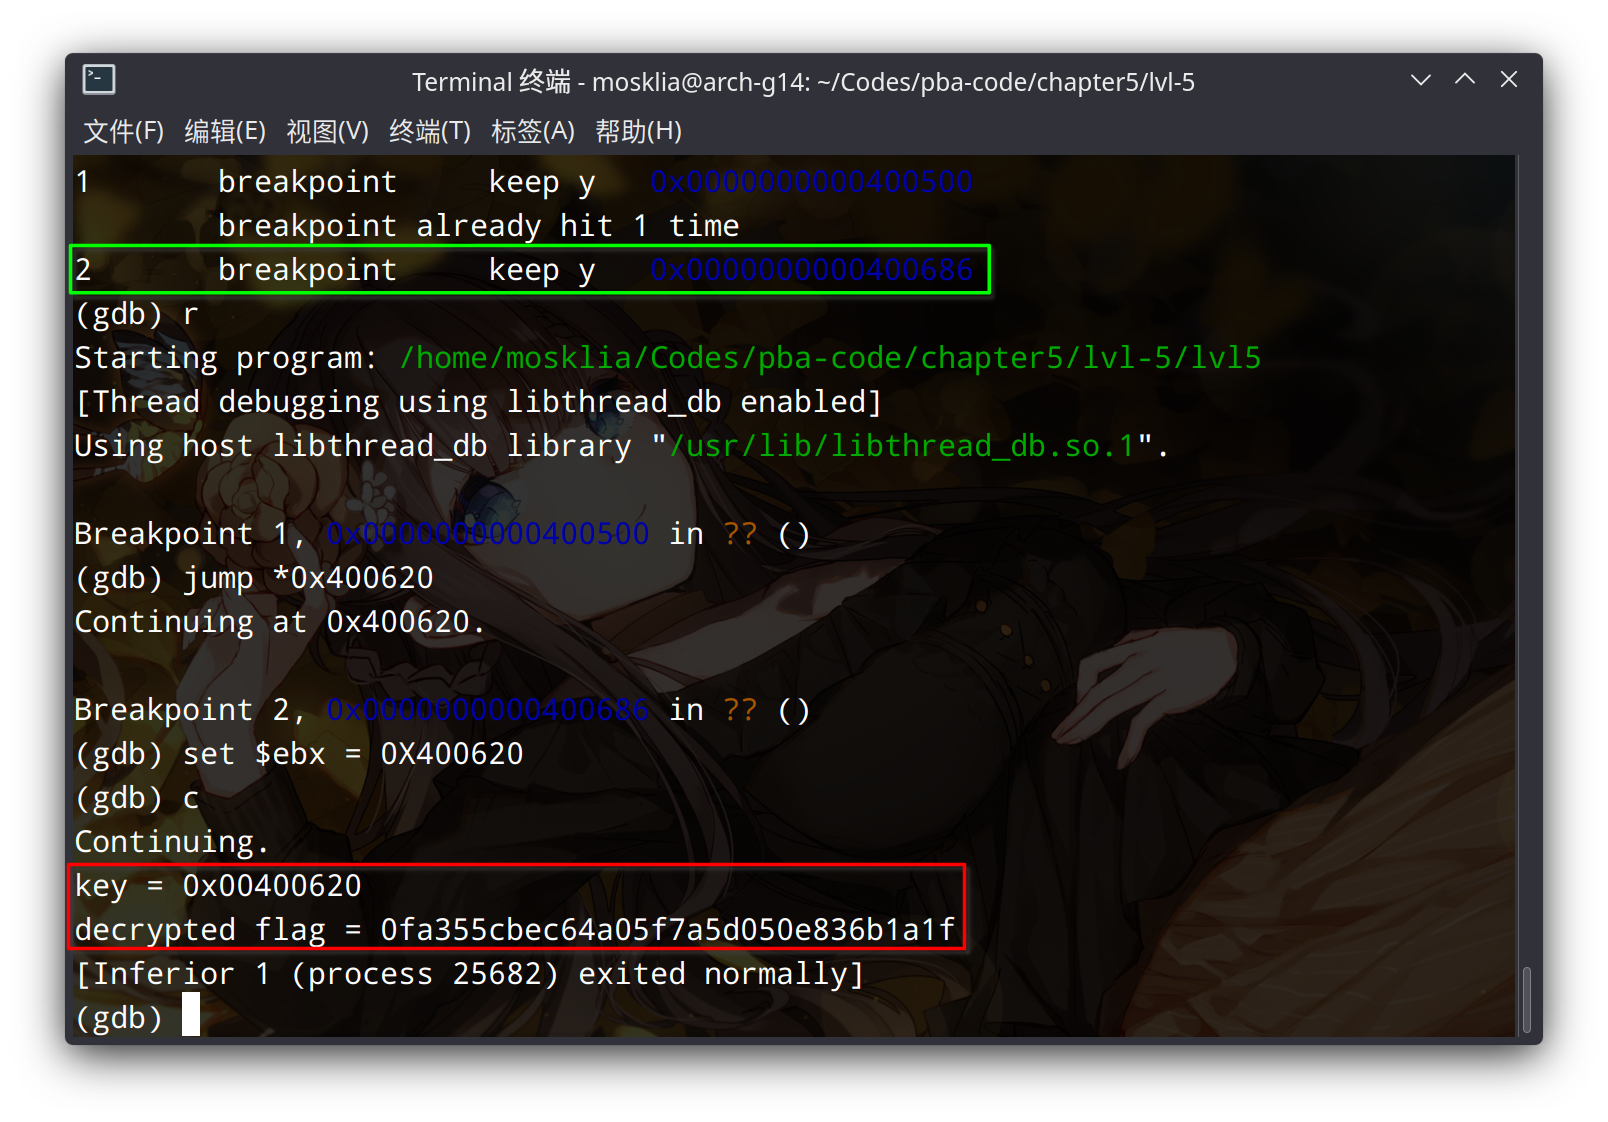
\includegraphics[width=0.4\textwidth]{pics/lvl5-gdb-2.png}
        \end{center}

        这一次得到了看起来像那么回事的 flag。验证一下,发现确实是 Level 5 的 flag,于是本关通关,capture the flag!
    
    \end{frame}

    \section{Level 6}

    \begin{frame}[fragile]
        \frametitle{Level 6}
        \framesubtitle{提示}
    
        \mintinline{text}{oracle} 给出的提示为:

        \begin{minted}{text}
            Find out what I expect, then trace me for a hint
                    找到我想要的,然后追踪我以获取提示
        \end{minted}
    
    \end{frame}

    \begin{frame}[fragile]
        \frametitle{Level 6}
        \framesubtitle{运行前检查}
    
        通过运行 \mintinline{text}{strings},可以看到以下内容:

        \begin{minted}{text}
            ......
            DEBUG: argv[1] = %s
            get_data_addr
            ......
        \end{minted}

        \pause 可以看出,程序肯定是需要使用一个命令行参数的。

        再运行 \mintinline{text}{nm},基本可以验证此猜想:

        {
            \scriptsize
            \begin{minted}[highlightlines={5,7}]{text}
                w __gmon_start__
                U __libc_start_main@GLIBC_2.2.5
                U __printf_chk@GLIBC_2.3.4
                U putchar@GLIBC_2.2.5
                U setenv@GLIBC_2.2.5
                U __sprintf_chk@GLIBC_2.3.4
                U __stack_chk_fail@GLIBC_2.4
                U strcmp@GLIBC_2.2.5
            \end{minted}
        }
    
    \end{frame}

    \begin{frame}[fragile]
        \frametitle{Level 6}
        \framesubtitle{带参数运行}
    
        合理猜测,需要的参数是 \mintinline{text}{get_data_addr},并且运行时会有有用的信息写入环境变量。

        于是使用 \mintinline{text}{ltrace}:

        {
            \begin{minted}[highlightlines={4}]{text}
                ......
                [0x40063d] strcmp("get_data_addr", "get_data_addr") = 0
                [0x40076c] __sprintf_chk(0x7ffc6854af90, 1, 1024, 0x400937) = 8
                [0x400783] setenv("DATA_ADDR", "0x4006c1", 1)    = 0
                ......
            \end{minted}
        }

        于是我们拿到了``数据''的地址``0X4006C1''。
    
    \end{frame}

    \begin{frame}[fragile]
        \frametitle{Level 6}
        \framesubtitle{反汇编}
    
        首先使用 \mintinline{text}{readelf} 确认该地址所处的节:

        {
            \scriptsize
            \begin{minted}{text}
                There are 29 section headers, starting at offset 0x1190:

                节头:
                  [号] 名称              类型             地址              偏移量
                       大小              全体大小          旗标   链接   信息   对齐
                ......
                  [14] .text             PROGBITS         00000000004005f0  000005f0
                       0000000000000312  0000000000000000  AX       0     0     16         
                ......
            \end{minted}
        }

        发现这个地址位于代码节中。
    
    \end{frame}

    \begin{frame}[fragile]
    
        然后反汇编代码节:

        {
            \scriptsize
            \begin{minted}[highlightlines={4,10}]{text}
                ......
                4006b8:	8b 44 24 24          	mov    eax,DWORD PTR [rsp+0x24]
                4006bc:	83 f8 00             	cmp    eax,0x0
                4006bf:	74 10                	je     4006d1 <__gmon_start__@plt+0xf1>
                4006c1:	2e 29 c6             	cs sub esi,eax
                4006c4:	4a 0f 03 a6 ee 2a 30 	rex.WX lsl rsp,WORD PTR [rsi+0x7f302aee]
                4006cb:	7f 
                4006cc:	ec                   	in     al,dx
                4006cd:	c8 c3 ff 42          	enter  0xffc3,0x42
                4006d1:	48 8d ac 24 90 01 00 	lea    rbp,[rsp+0x190]
                ......
            \end{minted}
        }

        发现 0X4006C1 到 0X4006CF 之间的内容似乎总是被跳过,并且 GDB 的跳转也证实,直接跳转到这里会导致崩溃。

        联系到这段范围内正好有 16 个字节(和 flag 为 32 个字符的字符串相对应),大胆猜测这一段的内容就是最终的 flag。
    
    \end{frame}

    \begin{frame}[fragile]
        \frametitle{Level 6}
        \framesubtitle{Capture the Flag}
    
        把这一段范围内的数据单独拿出来,得到:\pause

        \begin{minted}{text}
            2e29c64a0f03a6ee2a307fecc8c3ff42 
        \end{minted}

        \pause 验证发现这就是 Level 6 的 flag。Capture the flag!
    
    \end{frame}

    \section{所有 flags}

    \begin{frame}
        \frametitle{所有 flags}
    
        最后,这里列出了所有关卡的 flag:

        \begin{center}
            \ttfamily
            \begin{tabular}{cc}
                \hline
                Level & flag \\ \hline
                lvl1 & 84b34c124b2ba5ca224af8e33b077e9e \\
                lvl2 & 034fc4f6a536f2bf74f8d6d3816cdf88 \\
                lvl3 & 3a5c381e40d2fffd95ba4452a0fb4a40 \\
                lvl4 & 656cf8aecb76113a4dece1688c61d0e7 \\
                lvl5 & 0fa355cbec64a05f7a5d050e836b1a1f \\
                lvl6 & 2e29c64a0f03a6ee2a307fecc8c3ff42 \\
                lvl7 & 0f25e512a7763eefb7696b3aeda1f964 \\
                lvl8 & 2235a6b2123404469f4abce71b1dd29f \\ \hline
            \end{tabular}
        \end{center}
    
    \end{frame}
\end{document}